%\section[Dynamic Time Warping Tutorial Paper]{Let's do the Time Warp again!}
\section[Dynamic Time Warping Tutorial Paper]{Revisiting Dynamic Time Warping -- A practical tutorial in Python on North Sea field data}

\paragraph{Abstract:} This tutorial revisits Dynamic Time Warping for geoscientific applications.  This algorithm can be used to match arbitrary time-series, which is applicable to 4D time shifts, seismic-well ties, well-to-well ties, and seismic pre- and post-stack migration.  DTW is notorious to be computationally slow and expensive, while under-performing on seismic field data.  We show that a choice of similarity measures, optimization, and constraints can both speed up calculation and significantly improve results.  We show a full implementation in Python code on 4D seismic traces recorded over 10 years apart. Moreover, we explore recent developments in DTW and the significance to machine learning metrics

\subsection*{Key points:}
\begin{itemize}
    \item Tutorial paper shows full python code for \acl{dtw}
    \item Introduces Huber loss for geoscience problems
    \item Shows LB\_Keogh as constraint for seismic warping
    \item Aligns traces well despite large discrepancy
\end{itemize}


{\vfill\hfill\newline\fbox{\parbox{.97\textwidth}{\fullcite{dramsch2019dtw}}}}

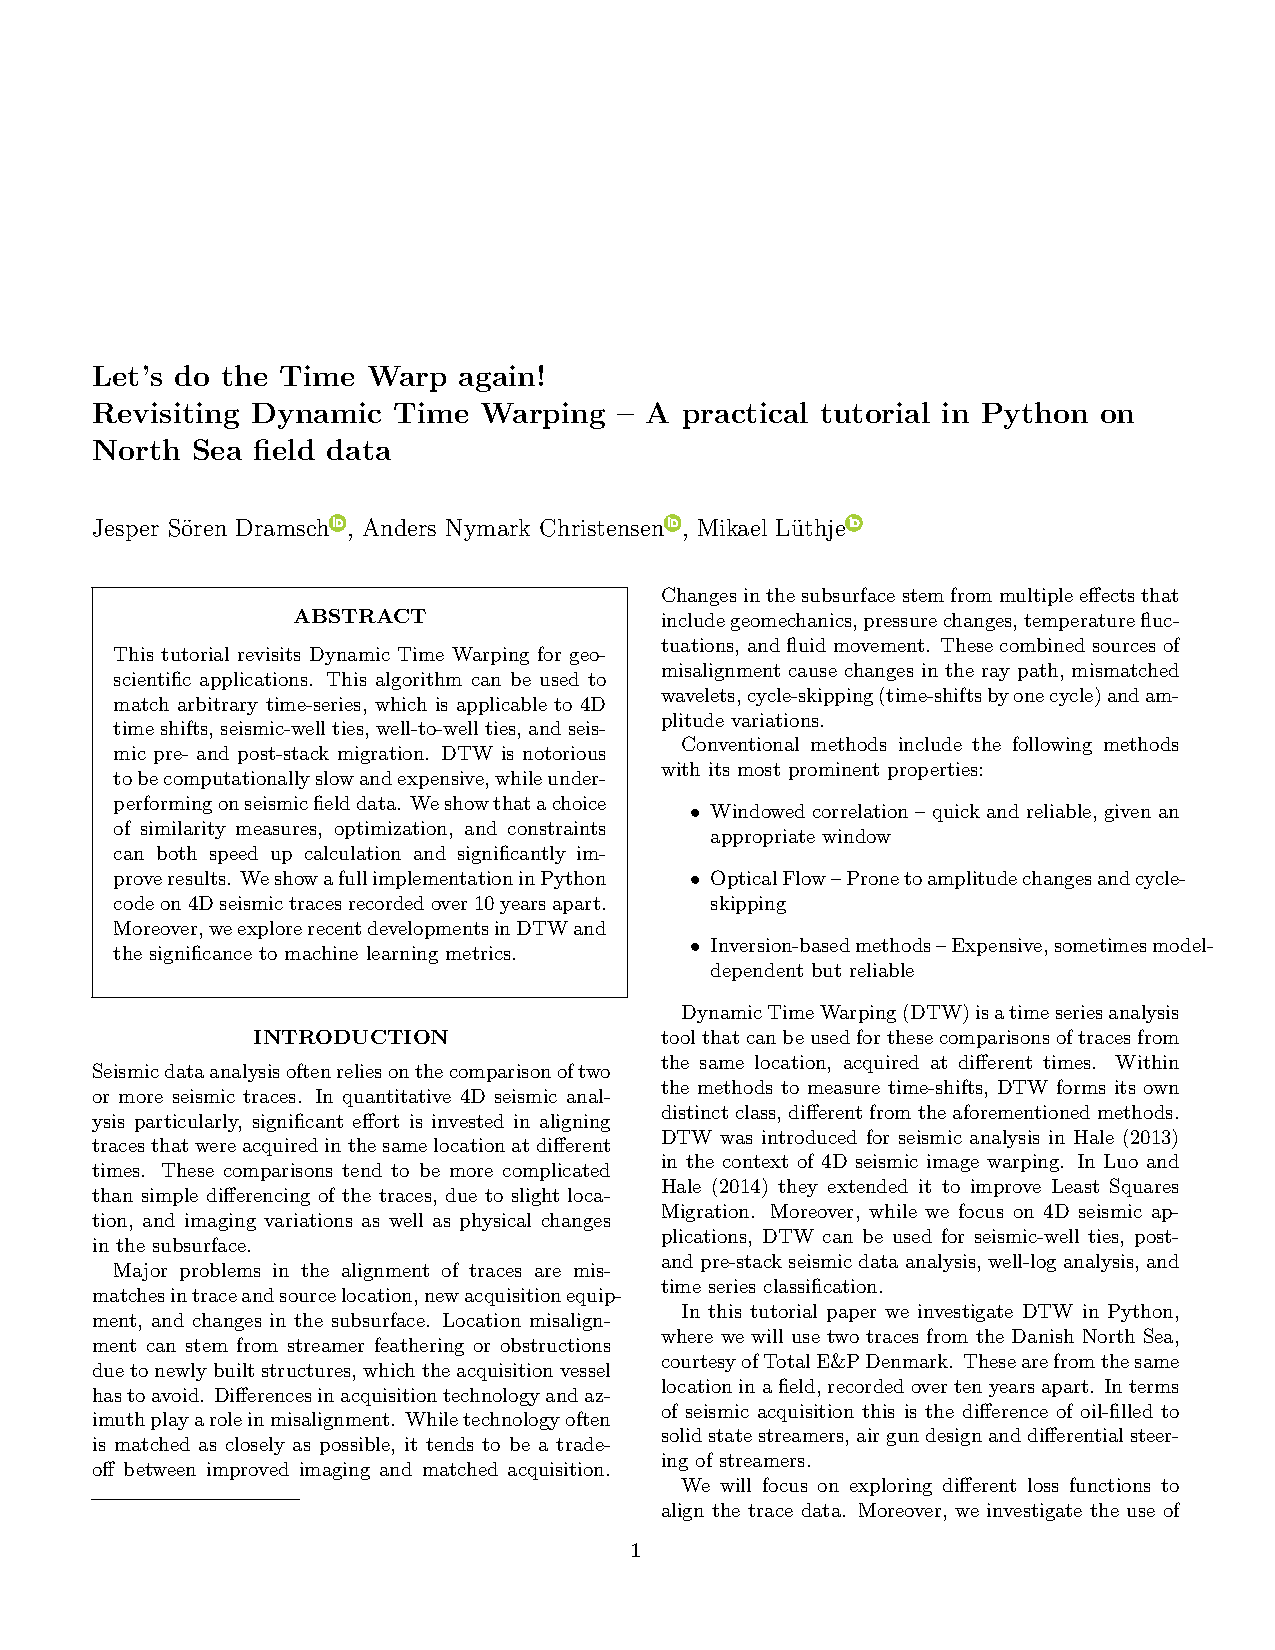
\includepdf[pages={1-9},pagecommand={},width=1.2\textwidth,offset=0.7cm 0.1cm]{papers/2019.4}